\documentclass[a4paper,UTF8]{ctexart}
\usepackage{graphicx}
\usepackage{subfig}
\usepackage{float}
\usepackage{geometry}
\usepackage{fancyhdr}
\geometry{papersize={20cm,15cm}}
\geometry{left=1cm,right=2cm,top=2cm,bottom=2cm}
\title{NNLM研究分析}
\author{王令博}
\date{\today}

\pagestyle{fancy}
\lhead{\author{王令博}}
\chead{\date}
\rhead{152xxxxxxxx}
\lfoot{}
\cfoot{\thepage}
\rfoot{}
\begin{document}
    \maketitle
    \section{你好世界}
    \subsection{NNLM}
    你好,今天介绍NNLM模型,这是第一个神经网络语言模型,主要用于语言建模,而词向量是它的一个副产物,如图\ref{fig:NNLM}是它的网络结构
    \begin{figure}[!t]
        \centering
        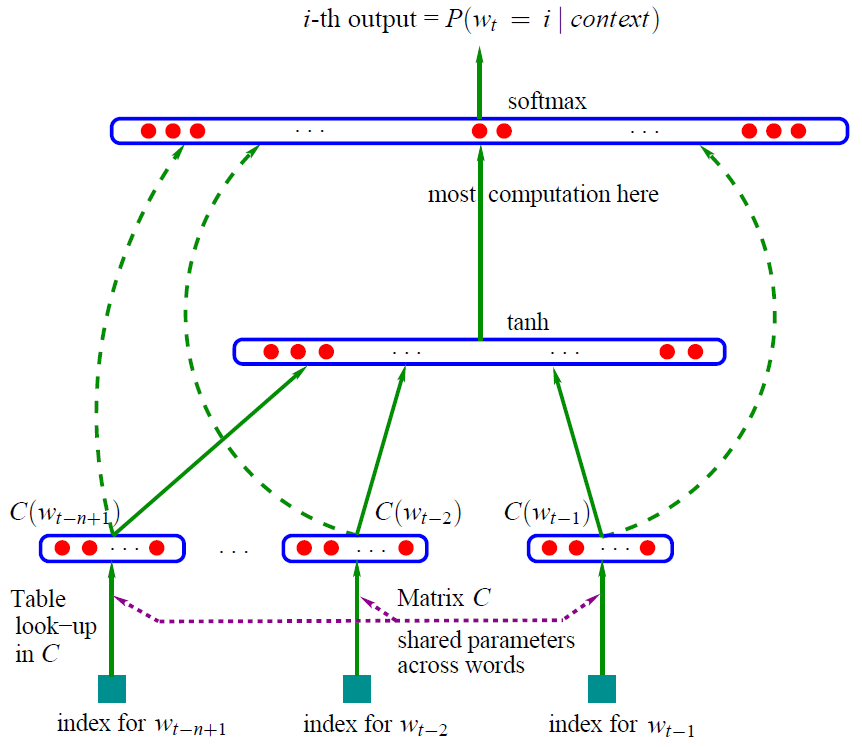
\includegraphics[width=4in]{img/NNLM.jpg}
        \caption{NNLM模型结构}
        \label{fig:NNLM}
    \end{figure}
    Learning to Navigate in Cities Without a Map \cite{mirowski2018learning}.
    有关svm论文 \cite{2007LIBSVM}。
    \bibliography{test}
    \bibliographystyle{ieeetr}
    
\end{document}